\chapter{Lernziele}\label{Lernziel}\label{Ziele}

Eine klassische Situation in deutschen Klassenzimmern: Der Lehrer gibt eine Schulaufgabe heraus, Notenschnitt unterirdisch. \say{Aber das habe ich Euch doch tausendmal erklärt!}, wie könne es dann sein, dass die gesamte Klasse Aufgabe 5 nicht beantworten konnte? Die lerntheoretische Strömung des \emph{Konstruktivismus} ($\to$ \cref{Konstruktivismus}) hat dafür eine einfache Erklärung: Etwas zu lernen erfordert eine aktive Konstruktion des Lerninhalts und damit verbundener Kompetenzen durch den Lernenden. Lehr- und Lernziele müssen also nicht übereinstimmen (siehe auch $\to$ \cref{EVA}).

\section{Lernen ordnen: Zum Begriff des Lernziels}
Jedes planm\"{a}{\ss}ige Handeln erfordert eine Zielsetzung:
So hat sich in der lerntheoretisch orientierten Unterrichtsforschung im Laufe der Zeit der Gedanke
der Zielformulierung durchgesetzt.
\mip
Der Begriff {\bf Lernziel} deutet dabei auf ein Endverhalten
der Sch\"{u}ler hin ($\to$ Operationalisierung). Es geht zun\"{a}chst weniger um die Art oder die Methodik
des Lernprozesses.
\mip
Ein Weg kann klarer ausgew\"{a}hlt und leichter beschritten werden,
wenn das Ziel bekannt ist.

\begin{itemize}
	\item Lernziele bilden f\"{u}r den Lehrenden den entscheidenden Rahmen f\"{u}r die
	Unterrichtsplanung, -umsetzung und -bewertung.
	\item Lernziele geben den Lernenden eine Orientierung über die von ihnen regelmäßig erwarteten Handlungsmuster und Lernerfolge.
	\item In Lernzielen werden die Erwartungen einer Gesellschaft
	(einschlie{\ss}lich Wirtschaft, Verb\"{a}nde, Kirchen, Hochschulen) an
	die Institution ,,Schule'' formuliert.
	\item Traditionen, neue Entwicklungen, Weltanschauungen oder
	Ideologien schlagen sich in den Lernzielen nieder.
	Beispiele: NewMaths, Umweltbewegung, Europa.
	\item
	Sie spiegeln deshalb den st\"{a}ndigen gesellschaftlichen
	Wechselprozess aus Bewahrung und Ver\"{a}nderung wieder.
%	\item
%	Im Begriff ,,Lernziel'' begegnen sich zwei grundlegende
%	Dimensionen von Unterricht:
%	
%	\begin{itemize}
%		\item
%		Auftrag zur Bildung der Pers\"{o}nlichkeit
%		(Anthropologische oder personale Dimension)
%		\item
%		Vermittlung fach(wissenschaft)licher Inhalte (Sachliche
%		oder inhaltliche Dimension)
%	\end{itemize}
\end{itemize}

\section{Funktionen von Lernzielen}
\begin{itemize}
	\item Lernziele sind -- gemeinsam mit den Lernvoraussetzungen -- gedanklicher Ausgangspunkt jeder Unterrichtsplanung ($\to$ \cref{Entwurf}). Schematisch dargestellt: \begin{equation*}
		\text{Lernvoraussetzungen} \longrightarrow \text{Unterrichtliches Handeln} \longrightarrow \text{Lernziele.}
	\end{equation*}
	\item Lernziele ermöglichen die Evaluation und Reflexion von Unterricht. Die Erreichung der Lernziele durch die Lernenden ist hierbei das Gütekriterium (und nicht etwa die vollständige und fachlich korrekte Darstellung durch die Lehrkraft).
	\item Lernziele stellen in den Mittelpunkt den Lernprozess der
	Sch\"{u}ler und nicht die Fachinhalte (Lerninhalte) oder
	die Unterrichtsmethodik (Lehrziele).
	\item
	Lernziele stellen ein Instrument f\"{u}r die Diskussion \"{u}ber
	schulische Erziehung und Unterricht bereit und bilden
	daher eine M\"{o}glichkeit zur Verst\"{a}ndigung von Lehrern,
	Sch\"{u}lern, Eltern, Didaktikern, Bildungspolitikern
	(Beispiel: Weltanschaulicher Unterricht, Sexualkunde).
	\item
	Der normative Charakter von Lernzielen erm\"{o}glicht es, den
	gesellschaftlichen Konsens \"{u}ber die Schule in den Unterricht zu
	transportieren. Lehrpl\"{a}ne (in Bayern) werden vom Kultusministerium verordnet
	und im Amtsblatt ver\"{o}ffentlicht. Die derzeit gültige Version ist der LehrplanPlus, der unter \url{lehrplanplus.bayern.de} abrufbar ist.
\end{itemize}

\begin{uea}
	Bringe folgende drei Ziele von Physikunterricht in eine hierarchische Ordnung:
	\begin{itemize}
		\item Einen Stromkreis aus Lampe, Batterie und Schalter aufbauen können.
		\item Ein allumfassend gebildeter, naturwissenschaftlich denkender Mensch werden.
		\item Die Newton'schen Axiome wiedergeben, an Beispielen erläutern und in Alltagsbeispielen anwenden können. 
	\end{itemize}
	Worin unterscheiden sich die angegebenen Ziele?
\end{uea}

\section{Lernzielebenen}

Lernziele lassen sich hierarchisch danach ordnen, über welche zeitliche Tragweite sie für die Unterrichtsplanung relevant sind. Eine ausführliche Darstellung der Lernzielebenen nach Westphalen (1979) findet sich bei \textcite{KircherGirwidzHaussler1} auf den Seiten 90 ff. Hier eine kurze Übersicht:

\begin{enumerate}
	\item \textbf{Leitziele:} Oberste, fächerübergreifende Ebene pädagogischer Aufgaben und Absichten, siehe $\to$ \href{https://www.gesetze-bayern.de/Content/Document/BayVerf-131}{Art. 131 BV}, $\to$ \href{https://www.gesetze-bayern.de/Content/Document/BayEUG-1}{Art. 1 BayEUG}.
	\begin{beisp2}
		Studierf\"{a}higkeit, Berufsf\"{a}higkeit, Allgemeinbildung, Bew\"{a}ltigung der Lebenswelt, gesellschaftliche Verantwortung.
	\end{beisp2}

	\item \textbf{Richtziele:} Genauere, teilweise fachspezifische Ausformulierungen der Leitziele, siehe $\to$ Fachprofil des Fachs Physik im LehrplanPlus.
	\begin{beisp2}
		Förderung des Verständnisses naturwissenschaftlicher Methoden und Denkweisen, Entwicklung von Problemlösungsfähigkeiten, Verständnis der Rolle der Physik in der Gesellschaft.
	\end{beisp2}


	\item \textbf{Grobziele} beschreiben eindeutig, aber nicht im Detail, die angestrebten Lernergebnisse innerhalb eines Faches. Denke bei einem Grobziel an ein Lernziel mehrerer Unterrichtseinheiten. Du findest diese durch die Gesamtschau des Fachlehrplans.

	\begin{beisp2}
		aus dem LPP Ph9: Verständnis der Energieerhaltung, Anwendung physikalischer Modelle, Bewertung gesellschaftlicher Auswirkungen
	\end{beisp2}

	\item \textbf{Feinziele (auch Unterrichtsziele, Teilziele)} differenzieren den Unterricht in kleinste Einzelziele. Du erhältst sie aus einzelnen, im Lehrplan angegebenen Kompetenzerwartungen. Ggf. musst Du diese noch konkretisieren.

	\begin{beisp2}
		aus dem LPP Ph9: Die Schülerinnen und Schüler nutzen das Prinzip der Energieerhaltung, um bei Energieumwandlungen mechanische Energieformen quantitativ zu bilanzieren und Größen zu berechnen.
	\end{beisp2}
\end{enumerate}

Diese Unterteilung ist nicht vollständig trennscharf. Für Deine Unterrichtsvorbereitung ($\to$ \cref{Entwurf}) sind vor allem Grob- und Feinziele relevant, wobei Du Leit- und Richtziele im Hinterkopf behältst. Im schriftlichen Unterrichtsentwurf geben Sie die Ebenen 3 und 4 an.

\section{Lernzieltaxonomien und Operationalisierung}

\begin{table}[ht] \tiny
\begin{tabular}{l|l|l|l|l|l|l}
 \multirow{2}{*}{Dimension \NL des Wissens}                 & \multicolumn{6}{c}{Dimension kognitiver Prozesse}                                        \\
                  & 1. Erinnern & 2. Verstehen & 3. Anwenden & 4. Analysieren & 5. Beurteilen & 6. Erschaffen \\ \hline
 A. Faktenwissen  &             &              &             &                &              &               \\ \hline
 B. Konzeptwissen &             &              &             &                &              &               \\ \hline
 C. Prozesswissen &             &              &             &                &              &               \\ \hline
 D. Metakognition &             &              &             &                &              &              
\end{tabular}\caption{Darstellung der Taxonomie nach Anderson und \textcite{Krathwohl}.}\label{tab:krathwohl}
\end{table}

Lernziele lassen sich nach verschiedenen Dimensionen des Gesamtspektrums menschlicher Verhaltensweisen einordnen. Die darauf aufbauenden Klassifizierungen hei{\ss}en Taxonomien (Einordnung, vgl.\ z.B.\ Biologie). Die bekannteste ist wohl die Taxonomie nach \textcite{Bloom}. Hier dargestellt wird die darauf aufbauende Taxonomie nach Anderson und \textcite{Krathwohl}.

Die Taxonomie weist zwei Dimensionen auf, die \emph{Dimension des Wissens} und die \emph{Dimension kognitiver Prozesse}, da die kognitiven Prozesse der Auseinandersetzung mit dem Lerngegenstand auf jeder Ebene auf Wissen im Hinblick auf den Lerngegenstand zurückgreifen.

\subsection{Zur Dimension des Wissens}
\begin{enumerate}[label=\Alph*.]
	\item \textbf{Faktenwissen:} Die grundlegenden Elemente, die Schüler wissen müssen, um Probleme zu lösen.
	\item \textbf{Konzeptwissen:} Die Beziehungen zwischen den grundlegenden Elementen innerhalb einer größeren Struktur, durch die sie gemeinsam funktionieren.
	\item \textbf{Prozesswissen:} Wie man etwas macht, Forschungsmethoden, und Kriterien zur Auswahl von Techniken und Methoden der Problemlösung.
	\item \textbf{Metakognitives Wissen:} Wissen um sowie über die eigene Kognition.
\end{enumerate}

\subsection{Zur Dimension kognitiver Prozesse}
\begin{enumerate}
	\item \textbf{Erinnern:} Relevantes Wissen aus dem Langzeitgedächtnis abrufen.
	\item \textbf{Verstehen:} Die Bedeutung von Lerninformationen bestimmen und mündlich, schriftlich, graphisch darstellen.
	\item \textbf{Anwenden:} Ein Verfahren in einer bestimmten Situation anwenden.
	\item \textbf{Analysieren:} Material in seine Bestandteile zerlegen und deren wechselseitige Beziehung und Zusammensetzung zum Ganzen erörtern.
	\item \textbf{Beurteilen:} Werturteile auf Grundlage von Kriterien und Standards fällen.
	\item \textbf{Erschaffen:} Elemente zu einem neuen Ganzen zusammensetzen oder ein Produkt entwickeln.
\end{enumerate}

\begin{uea}
	Ordne folgende Lernziele den Bereichen in \cref{tab:krathwohl} zu.
	\begin{enumerate}[label=\alph*.]
		\item Die Schüler können den Ablauf eines Experiments in seine einzelnen Schritte zerlegen und die Bedeutung jedes Schrittes im Kontext der Energieerhaltung erläutern.
		\item Die Schüler können mithilfe des Energieerhaltungssatzes erklären, wie Energie in geschlossenen Systemen erhalten bleibt.
		\item Die Schüler können ihre eigenen Denkprozesse beim Lösen von Aufgaben zur Energieerhaltung reflektieren und geeignete Strategien entwickeln, um Probleme effizienter zu lösen.
		\item Die Schüler können das Prinzip der Energieerhaltung anwenden, um in mechanischen Prozessen Energieumwandlungen zu berechnen.
		\item Die Schüler können die grundlegenden Konzepte der Energieerhaltung und die verschiedenen Energieformen (z. B. kinetische Energie, potenzielle Energie) aufzählen.
	\end{enumerate}
	Entwirf dann drei weitere, eigene Lernziele zu Bereichen, die noch nicht belegt sind.
	
	\flushright\rotatebox{180}{\tiny Lösung: C4, A2, D6, B3, A1}
\end{uea}

\subsection{Operationalisierung}
Vielleicht ist Dir aufgefallen, dass die Beispiele in der vorigen Übungsaufgabe alle eine bestimmte Struktur besitzen: Sie beginnen mit \emph{Die Schüler können}, gefolgt von einem \emph{Operatorverb} wie erläutern, erklären, reflektieren, entwickeln, anwenden, aufzählen.

\mip
Auf diese Weise formulierte Lernziele nennt man \textbf{Operationalisierte Lernziele}. Sie geben das gewünschte Endverhalten der Schüler an und machen die in der Unterrichtsplanung angegebenen Lernziele somit abprüfbar. Du kannst aus dem Lernziel direkt Aktivitäten und Aufgaben ableiten. Auch Lernziele im LehrplanPlus werden operationalisiert angegeben, wobei zusätzlich zu den erworbenen Kompetenzen Inhalte angegeben werden.

\mip
Ein enges Verständnis von Operationalisierten Lernzielen findet man bei Mager und \textcite{Gagne}. Hier darf das Lernziel keinen Interpretations\-spielraum mehr zulassen. Dies wird bewerkstelligt durch folgende Bedingungen:
\begin{enumerate}
	\item	Benennung des Endverhaltens, das direkt beobachtbar sein muss ($\to$ Behaviorismus).
	\item	Eindeutige Bezeichnung des Gegenstandes, auf den sich Lernziel bezieht.
	\item	Beschreibung der Rahmenbedingungen, Voraussetzungen, Hilfsmittel (z.B.\ Formelsammlung, Taschenrechner).
	\item	Angabe eines Beurteilungsma{\ss}stabes  f\"{u}r das als ausreichend 	geltendes Verhalten.
\end{enumerate} 
Zentral ist die Verwendung von Operatorverben, die auf Lernzielebenen referieren ($\to$ Verbliste im \cref{A_Verbliste}).

\begin{beisp}
	\textbf{Klassisch (veraltet):} \\ 
	Der Sch\"{u}ler soll Aufbau und Wirkungsprinzipien eines
	Elektromotors verstehen.
	
	\mip
	\textbf{Operationalisiert (üblich):} \\
	Der Sch\"{u}ler soll das Modell eines Elektromotors aufbauen k\"{o}nnen,
	seine wichtigsten Teile benennen und ihre Funktion erkl\"{a}ren k\"{o}nnen.
	
	\mip
	\textbf{In Reinform (beinahe übertrieben, aber als Übung und für Unterrichts- und Prüfungsvorbereitung nützlich):} \\
	Der Sch\"{u}ler soll das Leybold-Modell eines Elektromotors
		innerhalb von 10 Minuten aufbauen und verschalten k\"{o}nnen, er
		soll weiter die Begriffe ,,Stator, Rotor, Kommutator'' im
		Modell zuordnen k\"{o}nnen und die Funktion jedes dieser Bauteile
		in zwei S\"{a}tzen beschreiben k\"{o}nnen, wobei zwei Fehler erlaubt
		sind.
\end{beisp}

%----------------------------------------eingefuegt Axel Enders 26.10.2023----------------------------------------------------------------------------------------- vormals Kapitel 6

\section{Bildungsstandards und die KMK}\label{KmK}
Die Kultusministerkonferenz (Ständige Konferenz der Kultusminister in der Bundesrepublik Deutschland, kurz \emph{KMK}) hat beschlossen, Bildungsstandards zu erarbeiten mit dem Ziel, die Einheitlichkeit und Vergleichbarkeit von Zeugnissen und Abschl{\"u}ssen zwischen den Bundesl{\"a}ndern zu vereinbaren und dadurch ein H{\"o}chstma{\ss} an Mobilit{\"a}t von Fachkr{\"a}ften innerhalb der Bundesrepublik zu erreichen und  zur Gleichwertigkeit der Lebensverh{\"a}ltnisse in ganz Deutschland beizutragen \autocite{KMK}. Die Bundesl{\"a}nder haben sich verpflichtet, diese Standards zu implementieren und anzuwenden. Diese (m{\"u}hsam errungenen) Bildungsstandards werden allgemein als nationale Kompetenzziele angesehen und sollen als Messlatte f{\"u}r den Erfolg des Schulunterrichts, u.a. im Fach Physik, dienen. Die aktuell gültigen Fassungen wurden für den Mittleren Schulabschluss 2024, für das Abitur 2020 veröffentlicht.
\mip
Mit dem Erwerb des mittleren Schulabschlusses oder des Abiturs verf{\"u}gen die Schüler {\"u}ber naturwissenschaftliche \emph{Kompetenzen} im Allgemeinen, und {\"u}ber physikalische Kompetenzen im Besonderen. Sie bestehen jeweils in der Kombination von Kenntnissen und Fähigkeiten, die auf diesen beruhen.  
\mip
\leftskip=0.5cm \rightskip=0.5cm {\emph{{\textbf{Definition von Kompetenzen}} nach \textcite{Weinert}: die bei Individuen verf{\"u}gbaren oder durch sie erlernbaren kognitiven F{\"a}higkeiten und Fertigkeiten, um bestimmte Probleme zu 
l{\"o}sen, sowie die damit verbundenen motivationalen, volitionalen und sozialen Bereitschaften und F{\"a}higkeiten, um die Probleml{\"o}sungen in variablen Situationen erfolgreich und verantwortungsvoll nutzen zu k{\"o}nnen.}} 
\mip
%  \tabto{12em} \hangindent=4.62cm
\leftskip=0cm \rightskip=0cm Die in den folgenden vier Kompetenzbereichen festgelegten Standards beschreiben die notwendige physikalische Grundbildung \autocite{KMKneu}. Die Kompetenz bereiche stimmen für den \textcolor{orange}{Mittleren Schulabschluss} und das \textcolor{blue}{Abitur} im Wesentlichen überein; Unterschiede sind farblich markiert.

\paragraph{Sachkompetenz:} Kenntnis naturwissenschaftlicher Begriffe,
Konzepte, Gesetzmäßigkeiten, Theorien und Verfahren verbunden mit der Fähigkeit, diese zu
beschreiben, zu erklären, sachgerecht zu nutzen und auf fach- und alltagsbezogene Sachverhalte zu übertragen.

\paragraph{Erkenntnisgewinnungskompetenz:} Kenntnis grundlegender
naturwissenschaftlicher Denk- und Arbeitsweisen verbunden mit der Fähigkeit, diese zu beschreiben, zu erklären, \textcolor{blue}{zu verknüpfen,um Erkenntnisprozesse nachvollziehen oder gestalten zu können} \textcolor{orange}{für Erkenntnisprozesse systematisch zu nutzen,} und deren Möglichkeiten und Grenzen zu reflektieren.

\paragraph{Kommunikationskompetenz:} Kenntnis von Fachsprache und
fachtypischen Darstellungen \textcolor{blue}{und Argumentationsstrukturen} verbunden mit der Fähigkeit, daraus fachbezogene Informationen
zu erschließen, diese adres\-saten- und situationsgerecht aufzubereiten und sich argumentativ
auszutauschen.

\paragraph{Bewertungskompetenz:} Kenntnis von fachlichen und überfachlichen Perspektiven und Bewertungsverfahren verbunden mit der Fähigkeit, \textcolor{blue}{diese zu nutzen, um Aussagen bzw. Daten anhand verschiedener Kriterien zu beurteilen, sich dazu begründet Meinungen zu bilden,} \textcolor{orange}{Handlungsoptionen anhand verschiedener Kriterien zu beurteilen,} um Entscheidungen auch auf ethischer Grundlage zu treffen, die Folgen abzuschätzen und Entscheidungsprozesse zu reflektieren.

Im \cref{A_kmk} sind diese Kompetenzbereiche weiter ausgeführt.

\begin{uea}
	Ordne die folgenden Teilaufgaben des Physikabiturs 2024 den Teilkompetenzen aus \cref{A_kmk} zu. Tipp: Es kann jeweils mehr als eine Teilkompetenz angesprochen werden.
	\bip
	\textbf{Aufgabengruppe 11 - 1}
	
	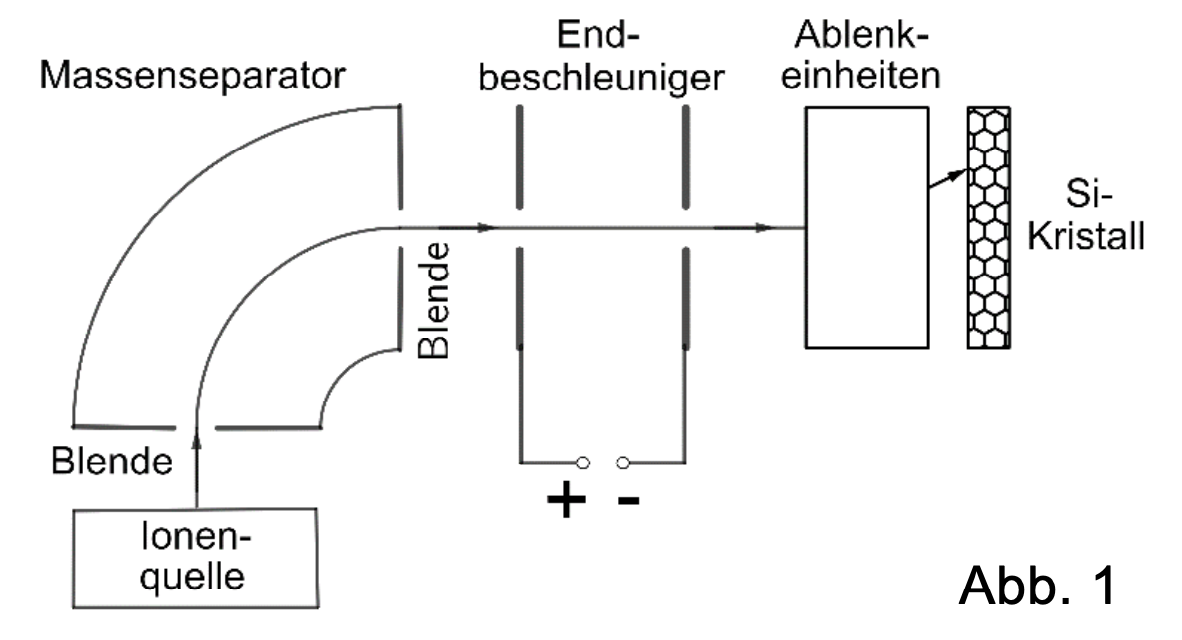
\includegraphics[width=.8\textwidth]{abitur.png}
	
	\begin{enumerate}[label = \arabic*)]
		\item Zur Herstellung von Computerchips werden Siliziumkristalle gezielt mit Fremdatomen durchsetzt. Abb. 1 zeigt den prinzipiellen Aufbau eines dafür verwendeten sogenannten Ionenimplanters. Die Ionen mit vernachlässigbarer Anfangsgeschwindigkeit werden in der Ionenquelle durch eine Spannung von $U = \SI{10}{\kilo\volt}$ vorbeschleunigt. Im Folgenden treffen einfach positiv geladene Arsen-Ionen \ce{^{75}As+} auf einen Siliziumkristall.
		\begin{enumerate}[label = \alph*)]
			\item Weisen Sie nach, dass die \ce{^{75}As+}-Ionen nach der Vorbeschleunigung eine Geschwindigkeit von \SI{1,6e5}{\metre\per\second} besitzen.
		\end{enumerate}
		Das Arsenpräparat in der Ionenquelle ist mit Antimon verunreinigt, weshalb sich im Ionenstrahl auch einfach positiv geladene Antimon-Ionen \ce{^{121}Sb+} befinden. Um diese aus dem Ionenstrahl zu entfernen, befindet sich hinter der Ionenquelle entweder ein Geschwindigkeitsfilter oder ein Massenseparator (s. Abb. 1).
		\begin{enumerate}[label = \alph*)]
			\setcounter{enumii}{1}
			\item Erläutern Sie mithilfe einer Skizze den Aufbau und die Funktionsweise eines Geschwindigkeitsfilters. Erklären Sie, dass die \ce{^{121}Sb+}-Ionen mit dessen Hilfe aus dem Ionenstrahl entfernt werden können. [...]
		\end{enumerate}
		\item Drahtloses Laden [...]
		\begin{enumerate}[label = \alph*)]
			\setcounter{enumii}{4}
			\item Es gibt Überlegungen, die drahtlose Ladetechnologie auch für Akkus von Elektroautos zu nutzen. Beschreiben Sie zwei Voraussetzungen, die hierfür geschaffen werden müssten, und beurteilen Sie, ob diese Ladetechnologie künftig eine große Rolle spielen wird.
		\end{enumerate}
	\end{enumerate}
\end{uea}




